\chapter{Fundamentos teóricos}\label{chap:fundamentos}

Este capítulo reúne los conceptos en los que se apoya el estudio experimental. Empieza
por las nociones de aprendizaje automático y aprendizaje profundo y pasa después al
aprendizaje federado: su algoritmo de referencia, sus variantes y los retos que
condicionan su evaluación. No se pretende repasar todo el campo de la inteligencia
artificial, sino dejar la base necesaria para entender el diseño de los experimentos y
la comparación entre \textit{frameworks}.

\section{Aprendizaje automático y aprendizaje profundo}\label{sec:ml-dl}

El aprendizaje automático es la rama de la inteligencia artificial que busca que un
sistema aprenda patrones a partir de datos, en lugar de seguir reglas programadas de
antemano \parencite{goodfellow2016deep}. En el enfoque supervisado, el más extendido en
este trabajo, el modelo se entrena con ejemplos etiquetados (pares de entrada y salida
esperada) y aprende una función que asocia cada nueva entrada con la salida correcta, en
tareas como la clasificación de imágenes o el reconocimiento de voz.

El aprendizaje profundo es la subárea que utiliza redes neuronales con varias capas,
capaces de aprender representaciones complejas de los datos \parencite{goodfellow2016deep}.
Durante el entrenamiento, el modelo genera una predicción para cada entrada, la compara
con la salida esperada mediante una función de pérdida y ajusta sus parámetros para ir
reduciendo ese error a lo largo de varias épocas. En clasificación, las dos métricas
habituales son la precisión (\textit{accuracy}), que indica la proporción de ejemplos
bien clasificados, y la pérdida (\textit{loss}), que cuantifica el error del modelo.

En visión por computador, las redes neuronales convolucionales han tenido un papel
destacado por su capacidad para procesar datos con estructura espacial. Entre ellas, las
redes residuales de \textcite{he2016deep} facilitaron el entrenamiento de redes muy
profundas gracias a las conexiones residuales; su arquitectura, ResNet, se emplea en
este trabajo como modelo común para comparar los \textit{frameworks}.

\section{Del entrenamiento centralizado al aprendizaje federado}\label{sec:centralizado-distribuido}

Desde un punto de vista técnico conviene distinguir tres enfoques de entrenamiento que a
menudo se confunden. El entrenamiento centralizado es el más directo: todos los datos se
reúnen en una misma infraestructura y el modelo se entrena sobre el conjunto completo, lo
que simplifica el control del experimento y la evaluación. El entrenamiento distribuido
reparte la carga de cálculo entre varios nodos para acelerar el proceso, pero suele
asumir que los datos pueden accederse o repartirse de forma controlada dentro de una
misma infraestructura. El aprendizaje federado, en cambio, parte de una premisa distinta:
la descentralización de los datos no es un recurso para ganar velocidad, sino una
condición impuesta por el problema \parencite{kairouz2021advances}.

Esta diferencia de premisa tiene consecuencias técnicas. En el aprendizaje federado el
servidor nunca observa los datos, solo modelos entrenados sobre ellos, de modo que la
distribución de los datos entre clientes deja de ser una decisión del diseñador y pasa a
ser un dato del problema, normalmente desconocido y desigual. La
Figura~\ref{fig:centralizado-federado} contrasta los dos esquemas extremos: en el
centralizado los datos se trasladan al servidor, mientras que en el federado permanecen
en cada cliente y solo se intercambian el modelo global y los modelos locales
resultantes.

\begin{figure}[htbp]
  \centering
  \begin{subfigure}[b]{0.48\textwidth}
    \centering
    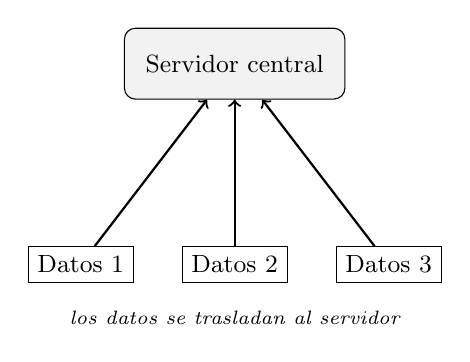
\begin{tikzpicture}[scale=0.85, every node/.style={font=\small}]
      \node[draw, rounded corners, fill=gray!10, minimum width=2.8cm, minimum height=0.9cm] (s) at (0,3) {Servidor central};
      \node[draw, minimum width=1.2cm] (d1) at (-2.3,0) {Datos 1};
      \node[draw, minimum width=1.2cm] (d2) at (0,0)    {Datos 2};
      \node[draw, minimum width=1.2cm] (d3) at (2.3,0)  {Datos 3};
      \draw[->, thick] (d1) -- (s);
      \draw[->, thick] (d2) -- (s);
      \draw[->, thick] (d3) -- (s);
      \node[font=\scriptsize\itshape] at (0,-0.8) {los datos se trasladan al servidor};
    \end{tikzpicture}
    \caption{Entrenamiento centralizado.}
    \label{fig:centralizado}
  \end{subfigure}\hfill
  \begin{subfigure}[b]{0.48\textwidth}
    \centering
    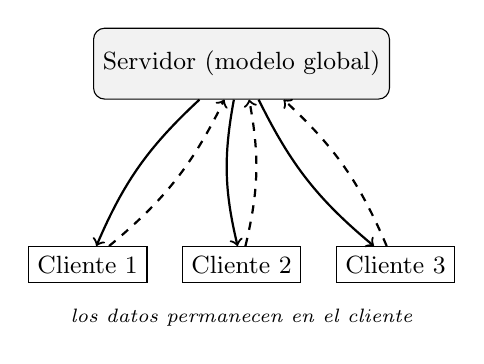
\begin{tikzpicture}[scale=0.85, every node/.style={font=\small}]
      \node[draw, rounded corners, fill=gray!10, minimum width=2.8cm, minimum height=0.9cm] (s) at (0,3) {Servidor (modelo global)};
      \node[draw, minimum width=1.2cm] (c1) at (-2.3,0) {Cliente 1};
      \node[draw, minimum width=1.2cm] (c2) at (0,0)    {Cliente 2};
      \node[draw, minimum width=1.2cm] (c3) at (2.3,0)  {Cliente 3};
      \draw[->, thick]         (s) to[bend right=12] (c1);
      \draw[->, thick, dashed] (c1) to[bend right=12] (s);
      \draw[->, thick]         (s) to[bend right=12] (c2);
      \draw[->, thick, dashed] (c2) to[bend right=12] (s);
      \draw[->, thick]         (s) to[bend right=12] (c3);
      \draw[->, thick, dashed] (c3) to[bend right=12] (s);
      \node[font=\scriptsize\itshape] at (0,-0.8) {los datos permanecen en el cliente};
    \end{tikzpicture}
    \caption{Aprendizaje federado.}
    \label{fig:federado}
  \end{subfigure}
  \caption{Comparación entre el entrenamiento centralizado, en el que los datos se
  reúnen en una infraestructura común, y el aprendizaje federado, en el que solo se
  intercambian el modelo global (línea continua) y los modelos locales entrenados (línea
  discontinua). Elaboración propia a partir de \textcite{mcmahan2017communication} y
  \textcite{kairouz2021advances}.}
  \label{fig:centralizado-federado}
\end{figure}

\section{Aprendizaje federado}\label{sec:fl}

El aprendizaje federado organiza el entrenamiento en torno a un servidor central y un
conjunto de clientes que conservan sus datos locales \parencite{mcmahan2017communication}.
El servidor coordina el proceso, mantiene el modelo global y agrega los modelos que
recibe; los clientes entrenan ese modelo con sus propios datos. Las siguientes
subsecciones describen cómo funciona una ronda y cuál es su algoritmo de referencia, las
variantes algorítmicas que lo extienden, los tipos de aprendizaje federado que se
distinguen y los retos que condicionan su evaluación.

\subsection{Funcionamiento: la ronda federada y el algoritmo \textit{FedAvg}}\label{sec:ronda}

El proceso arranca con un modelo global inicializado en el servidor. En cada ronda, el
servidor escoge un subconjunto de clientes y les envía el modelo actual; cada cliente lo
entrena con sus datos locales durante un número fijo de épocas y devuelve su modelo local
ya entrenado; el servidor combina esos modelos con una estrategia de agregación y obtiene
una nueva versión del modelo global \parencite{mcmahan2017communication}. El ciclo, que
recoge la Figura~\ref{fig:ronda-federada}, se repite hasta completar el número de rondas
previsto o hasta cumplir un criterio de parada.

\begin{figure}[htbp]
  \centering
  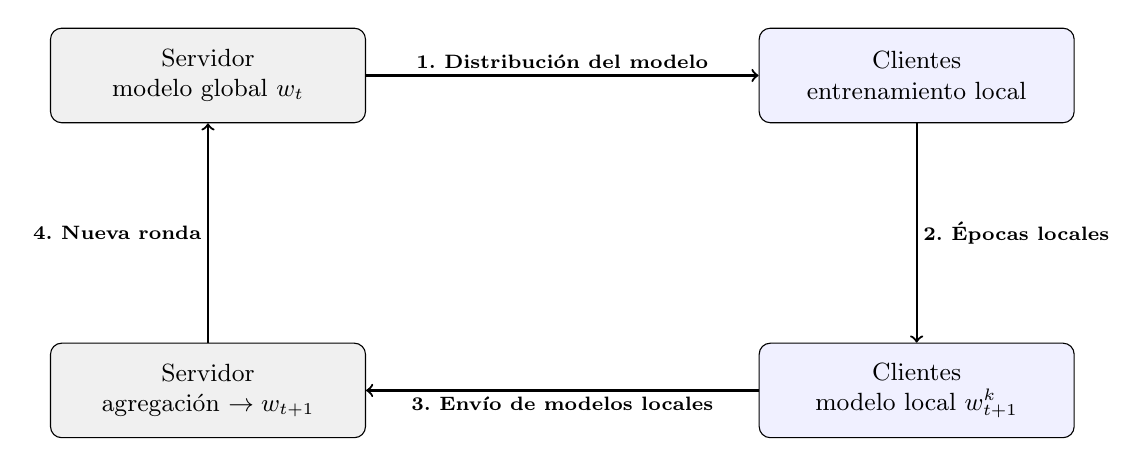
\begin{tikzpicture}[
      every node/.style={font=\small, align=center},
      caja/.style={draw, rounded corners, minimum width=4cm, minimum height=1.2cm, inner sep=4pt},
      servidor/.style={caja, fill=gray!12},
      cliente/.style={caja, fill=blue!6},
      paso/.style={font=\scriptsize\bfseries, fill=white, inner sep=2pt, midway}
    ]
    % Nodos en disposición 2x2 con amplia separación para evitar solapamientos
    \node[servidor] (g)  at (0,4) {Servidor\\ modelo global $w_t$};
    \node[cliente]  (lt) at (9,4) {Clientes\\ entrenamiento local};
    \node[cliente]  (up) at (9,0) {Clientes\\ modelo local $w_{t+1}^{k}$};
    \node[servidor] (ag) at (0,0) {Servidor\\ agregación $\to w_{t+1}$};
    % Aristas del ciclo (sentido horario) con etiquetas numeradas sobre fondo blanco
    \draw[->, thick] (g)  -- node[paso, above]{1.~Distribución del modelo} (lt);
    \draw[->, thick] (lt) -- node[paso, right]{2.~Épocas locales} (up);
    \draw[->, thick] (up) -- node[paso, below]{3.~Envío de modelos locales} (ag);
    \draw[->, thick] (ag) -- node[paso, left]{4.~Nueva ronda} (g);
  \end{tikzpicture}
  \caption{Ciclo de una ronda federada en \textit{FedAvg}: el servidor distribuye el
  modelo global, cada cliente lo entrena con sus datos locales, devuelve su modelo local
  entrenado y el servidor agrega esos modelos para generar una nueva versión del modelo
  global \parencite{mcmahan2017communication}.}
  \label{fig:ronda-federada}
\end{figure}

En este proceso intervienen varios conceptos. Una \textit{ronda federada} es una
iteración completa del ciclo de distribución, entrenamiento local, recepción de los
modelos y agregación. Una \textit{época local} indica cuántas veces recorre cada cliente
su conjunto de datos durante el entrenamiento. El \textit{tamaño de lote}
(\textit{batch size}) fija cuántos ejemplos se procesan antes de actualizar los
parámetros, y la \textit{tasa de aprendizaje} regula la magnitud de cada paso de
actualización. Su configuración influye directamente en el coste y la estabilidad del
entrenamiento: subir el número de épocas locales reduce la comunicación, pero puede
aumentar la divergencia entre clientes cuando sus datos son muy heterogéneos
\parencite{mcmahan2017communication}.

La terminología requiere una precisión adicional, ya que «actualización» se emplea a menudo de forma
ambigua. En sentido estricto, en cada ronda el servidor recibe de cada cliente su
\textit{modelo local} ya entrenado, es decir, el vector de pesos $w_{t+1}^{k}$ resultante
de aplicar varias épocas de entrenamiento al modelo global recibido. Esto contrasta con
otros esquemas en los que lo que se transmite es una \textit{actualización} entendida
como la diferencia (o gradiente acumulado) respecto al modelo de partida. El algoritmo de
referencia del aprendizaje federado, \textit{Federated Averaging}
(FedAvg)\label{sec:fedavg}, opera sobre los modelos locales: agrega los pesos
$w_{t+1}^{k}$ ponderándolos por el número de ejemplos de cada cliente, y es precisamente
la estrategia de agregación que se ejecuta dentro de la ronda descrita
\parencite{mcmahan2017communication}.

Formalmente, \textit{FedAvg} busca minimizar una función de pérdida global definida como
la media de las pérdidas locales, ponderada por el número de ejemplos de cada cliente.
Para $K$ clientes, donde el cliente $k$ dispone de $n_k$ ejemplos y
$n = \sum_{k=1}^{K} n_k$, el objetivo es:

\begin{equation}
  \min_{w} \; F(w) = \sum_{k=1}^{K} \frac{n_k}{n}\, F_k(w),
  \qquad
  F_k(w) = \frac{1}{n_k} \sum_{i \in \mathcal{P}_k} \ell\!\left(w; x_i, y_i\right),
  \label{eq:fedavg-objetivo}
\end{equation}

\noindent donde $F_k(w)$ es la pérdida media en el conjunto local $\mathcal{P}_k$ del
cliente $k$ y $\ell(\cdot)$ es la función de pérdida por ejemplo. En cada ronda $t$, el
servidor selecciona un subconjunto de clientes $S_t$, les envía el modelo global $w_t$ y
cada cliente realiza varias épocas de descenso de gradiente estocástico sobre sus datos,
con lo que obtiene su modelo local $w_{t+1}^{k}$. El servidor agrega después esos modelos
locales mediante el promedio ponderado por el número de muestras:

\begin{equation}
  w_{t+1} = \sum_{k \in S_t} \frac{n_k}{n_{S_t}}\, w_{t+1}^{k},
  \qquad
  n_{S_t} = \sum_{j \in S_t} n_j .
  \label{eq:fedavg-agg}
\end{equation}

De este modo, los clientes con más datos pesan proporcionalmente más en el modelo global
resultante. El procedimiento completo se resume en el pseudocódigo del
Código~\ref{cod:fedavg}, que separa la lógica del servidor de la del cliente
\parencite{mcmahan2017communication}.

% El listado de codigo es contenido verbatim-like y el etiquetado PDF/UA
% experimental (tagpdf) no lo procesa correctamente: descuadra el recuento de
% parrafos. Se suspende el etiquetado a su alrededor con \tagstop/\tagstart.
% La guarda \providecommand evita errores si el etiquetado no esta activo.
\providecommand{\tagstop}{}
\providecommand{\tagstart}{}
\tagstop
\begin{pythoncode}[title={Pseudocódigo de Federated Averaging (FedAvg)}, label={cod:fedavg}, list entry={\protect\numberline{\thelisting}Pseudocódigo de Federated Averaging (FedAvg)}]
# --- Servidor ---
inicializar modelo global w_0
para t = 0, 1, ..., T-1:
    S_t = seleccionar subconjunto de clientes
    para cada cliente k en S_t (en paralelo):
        w_local[k] = ClienteActualiza(k, w_t)      # modelo local entrenado
    # Agregacion: promedio ponderado de los MODELOS locales por n_k
    n_St = sumar n_k para todo k en S_t
    w_(t+1) = sumar (n_k / n_St) * w_local[k] para todo k en S_t
devolver w_T

# --- Cliente k ---
funcion ClienteActualiza(k, w):
    para cada epoca e = 1, ..., E:
        para cada lote b en datos_locales[k]:
            w = w - eta * gradiente(perdida(w, b))
    devolver w                                       # pesos locales actualizados
\end{pythoncode}
\tagstart

La sencillez de \textit{FedAvg} lo hace muy adecuado para experimentos comparativos: al
reducir la complejidad algorítmica, deja el foco en el comportamiento de los
\textit{frameworks} y en el consumo de recursos. Su rendimiento, eso sí, puede empeorar
cuando los datos se distribuyen de forma no~IID entre los clientes, porque los modelos
locales llegan a diferir bastante y dificultan la convergencia
\parencite{li2020federated}. Aun con esa limitación, sigue siendo la referencia frente a
la que se comparan métodos más sofisticados, y es el algoritmo que se emplea de manera
uniforme en todos los \textit{frameworks} evaluados en este trabajo.

\subsection{Variantes de \textit{FedAvg}}\label{sec:variantes}

El carácter de referencia de \textit{FedAvg} no impide reconocer sus limitaciones; de
hecho, ha servido de punto de partida a varias variantes que buscan mejorar su
convergencia, sobre todo en presencia de datos heterogéneos. La más directa es
\textit{Federated Proximal} (FedProx), propuesta por \textcite{li2020fedprox}, que
conserva el esquema de \textit{FedAvg} pero añade al entrenamiento local un término
proximal, es decir, una penalización que limita cuánto pueden alejarse los pesos locales
del modelo global recibido al inicio de la ronda. Con ello reduce la deriva de los
clientes cuando sus distribuciones difieren y tolera mejor la heterogeneidad de recursos,
al admitir que cada cliente realice una cantidad desigual de trabajo local.

Una segunda línea de mejora actúa sobre el lado del servidor. La familia de optimización
federada adaptativa \textit{Federated Optimization} (FedOpt), introducida por
\textcite{reddi2021adaptive}, generaliza \textit{FedAvg} sustituyendo el promedio simple
del servidor por un optimizador con momento y tasa de aprendizaje propios. Sus variantes
más conocidas, FedAdam y FedAdagrad, emplean en el servidor los optimizadores Adam y
Adagrad, respectivamente. Estas estrategias pueden acelerar la convergencia, pero
introducen hiperparámetros adicionales —la tasa de aprendizaje del servidor y un factor de
adaptabilidad— cuya configuración resulta delicada, un aspecto que reaparece en los
experimentos de flexibilidad de esta memoria (Sección~\ref{sec:flex-comparativa}).

Un tercer enfoque corrige de forma explícita la deriva entre clientes. \textit{SCAFFOLD},
propuesto por \textcite{karimireddy2020scaffold}, introduce variables de control que
estiman y compensan la divergencia de cada cliente respecto a la dirección global, lo que
mejora la convergencia con datos no~IID a costa de transmitir información adicional en cada
ronda. Estas variantes extienden \textit{FedAvg}, pero no lo sustituyen como referencia: en
este trabajo \textit{FedAvg} se mantiene como algoritmo común a los tres
\textit{frameworks} para preservar un escenario controlado, mientras que FedProx, FedOpt,
FedAdam y FedAdagrad intervienen únicamente como pruebas puntuales dentro del análisis de
flexibilidad (Capítulo~\ref{chap:resultados}).

\subsection{Tipos de aprendizaje federado}\label{sec:tipos}

El aprendizaje federado no designa un escenario único, sino una familia de
configuraciones que conviene distinguir, porque condicionan tanto el diseño del sistema
como su evaluación. Una primera clasificación atiende al tipo y número de participantes.
\textcite{kairouz2021advances} diferencian entre escenarios \textit{cross-device} y
\textit{cross-silo}. El primero reúne a un número muy elevado de dispositivos de usuario
final (teléfonos, tabletas o dispositivos del internet de las cosas), con disponibilidad
intermitente, recursos limitados y conexiones inestables; aquí el sistema debe tolerar
que solo participe una fracción de los clientes en cada ronda y que algunos abandonen a
mitad del proceso. El segundo se da cuando intervienen pocas entidades, más estables y
con mayor capacidad de cómputo, como hospitales, bancos o universidades, cada una con una
cantidad apreciable de datos y una infraestructura fiable; en este caso la participación
suele ser completa y el reto se desplaza hacia la heterogeneidad de las distribuciones y
hacia las garantías de seguridad entre organizaciones.

Una segunda clasificación atiende a cómo se reparten los datos en el espacio de
características. \textcite{yang2019federated} distinguen entre aprendizaje federado
horizontal, vertical y por transferencia. En el horizontal los clientes comparten el
mismo espacio de características pero poseen ejemplos distintos, como dos hospitales que
registran las mismas variables sobre pacientes diferentes. En el vertical los clientes
comparten parte de los individuos o entidades pero describen atributos distintos, como un
banco y una aseguradora que conocen a los mismos clientes desde dimensiones diferentes;
este caso exige alinear registros y suele recurrir a técnicas de cómputo seguro. El de
transferencia se aplica cuando difieren a la vez los ejemplos y las características, y
aprovecha el conocimiento de un dominio para mejorar otro relacionado.

Situar un experimento dentro de esta taxonomía es imprescindible para interpretar sus
resultados. El estudio que se desarrolla en esta memoria corresponde a un escenario
\textit{cross-silo} con aprendizaje federado horizontal: un número reducido de clientes
estables, simulados sobre una misma máquina, que comparten el espacio de características
de un mismo conjunto de imágenes y se reparten ejemplos distintos. Esta delimitación
permite mantener un escenario controlado y reproducible, en el que las diferencias
observadas pueden atribuirse al \textit{framework} y no a la configuración federada.

\subsection{Retos del aprendizaje federado}\label{sec:retos}

El aprendizaje federado hereda los problemas del aprendizaje automático y añade otros
propios de su naturaleza distribuida y descentralizada. El más característico es la
heterogeneidad de los datos\label{sec:noiid}. A diferencia del entrenamiento
centralizado, cada cliente solo observa una parte del problema, que puede ser desigual en
cantidad y en distribución. Cuando esas distribuciones difieren de un cliente a otro se
habla de datos no independientes e idénticamente distribuidos (no~IID), una situación
habitual en la práctica: dos usuarios de móvil generan datos muy distintos y dos
hospitales atienden a poblaciones con características clínicas diferentes
\parencite{kairouz2021advances}. Esta heterogeneidad afecta directamente al
entrenamiento, ya que un cliente que observa una porción sesgada del problema produce un
modelo local que se aleja del de los demás, lo que ralentiza la convergencia del modelo
global o lo vuelve menos estable \parencite{li2020federated}. A ella se suma la
heterogeneidad de recursos: no todos los clientes disponen de la misma capacidad de
cómputo, memoria o conexión, lo que desequilibra su participación y obliga a diseñar
sistemas tolerantes a esas diferencias. Por eso la forma de repartir los datos entre
clientes influye tanto en la evaluación de un sistema federado y debe describirse de
manera explícita en cualquier experimento.

Un segundo reto es el coste de comunicación. En cada ronda viaja información entre el
servidor y los clientes, y ese volumen crece con el tamaño del modelo y con el número de
participantes, hasta convertirse en el principal cuello de botella en escenarios con
muchos dispositivos o con conexiones limitadas. De hecho, reducir el número de rondas
necesarias y la información intercambiada fue una de las motivaciones originales de
\textit{FedAvg}, que aumenta el cómputo local de cada cliente para disminuir la frecuencia
de las comunicaciones \parencite{mcmahan2017communication,li2020federated}. Existe así un
compromiso entre cómputo local y comunicación que cada sistema resuelve de forma distinta.

El tercer frente, y uno de los más delicados, es la seguridad y la privacidad. Aunque los
datos originales no se transfieren, los modelos locales pueden filtrar información sobre
los datos que los generaron mediante ataques de inferencia o de reconstrucción, y un
cliente malicioso podría enviar modelos manipulados para degradar o sesgar el modelo
global. Para mitigar estos riesgos se han desarrollado técnicas complementarias como la
agregación segura, la privacidad diferencial o la detección de anomalías
\parencite{kairouz2021advances,bonawitz2019towards}. El aprendizaje federado
reduce la necesidad de centralizar datos, pero no resuelve por sí solo todos los
problemas de privacidad, lo que explica que algunos \textit{frameworks} incorporen de
serie estos mecanismos mientras que otros los dejan a cargo del desarrollador.


